\documentclass{report}

%* Packages Used

\usepackage[english]{babel}
\usepackage[utf8]{inputenc}

\usepackage{verbatim}
\usepackage{fancyvrb}

\usepackage{listings}
\usepackage{xcolor}


\usepackage{amsmath}
\usepackage{graphicx}
\usepackage{hyperref}
\usepackage{geometry}

%* Package settings
\hypersetup{
colorlinks  = true,
linkcolor   = black,
urlcolor    = red,
}

\newgeometry{
      top = 0.75in,
      bottom = 0.75in,
      left = 0.75in,
      right = 0.75in,
}

%* C style

\definecolor{mGreen}{rgb}{0,0.6,0}
\definecolor{mGray}{rgb}{0.5,0.5,0.5}
\definecolor{mPurple}{rgb}{0.58,0,0.82}
\definecolor{backgroundColour}{rgb}{0.95,0.95,0.92}

\lstdefinestyle{C_style}{
    backgroundcolor=\color{backgroundColour},   
    commentstyle=\color{mGreen},
    keywordstyle=\color{magenta},
    numberstyle=\tiny\color{mGray},
    stringstyle=\color{mPurple},
    basicstyle=\footnotesize,
    breakatwhitespace=false,         
    breaklines=true,                 
    captionpos=b,                    
    keepspaces=true,                 
    numbers=left,                    
    numbersep=5pt,                  
    showspaces=false,                
    showstringspaces=false,
    showtabs=false,                  
    tabsize=2,
    language=C
}

%* Preamble

\title{

\includegraphics[width=0.5\textwidth]{resources/feri_logo.png} \\
Activity Bot's Catch Game\\
\Large{University of Maribor}
}

\author{Bruno Silva\\
      \href{https://github.com/brunofavs/propeller_cath_game}{Github Repository}
      }

\setcounter{chapter}{1}

\begin{document}
\maketitle

\tableofcontents
\listoffigures
\pagebreak

\section{Introduction}

This project is based on 2 robots from \textit{Parallax} the \textit{Activity
Bots}, and the goal was to create a recreation of the kids game "The Catch".

There's one robot with a seeker algorithm and another one with a runner
algorithm. The seeker uses a pair of ultrasonic sensors to figure which
direction an incoming target is coming from. The runner robot is programmed to
run around in a pseudo-random way in the playing field in an open loop system.

\begin{figure}[h]
    \centering
    \begin{minipage}{0.45\textwidth}
        \centering
        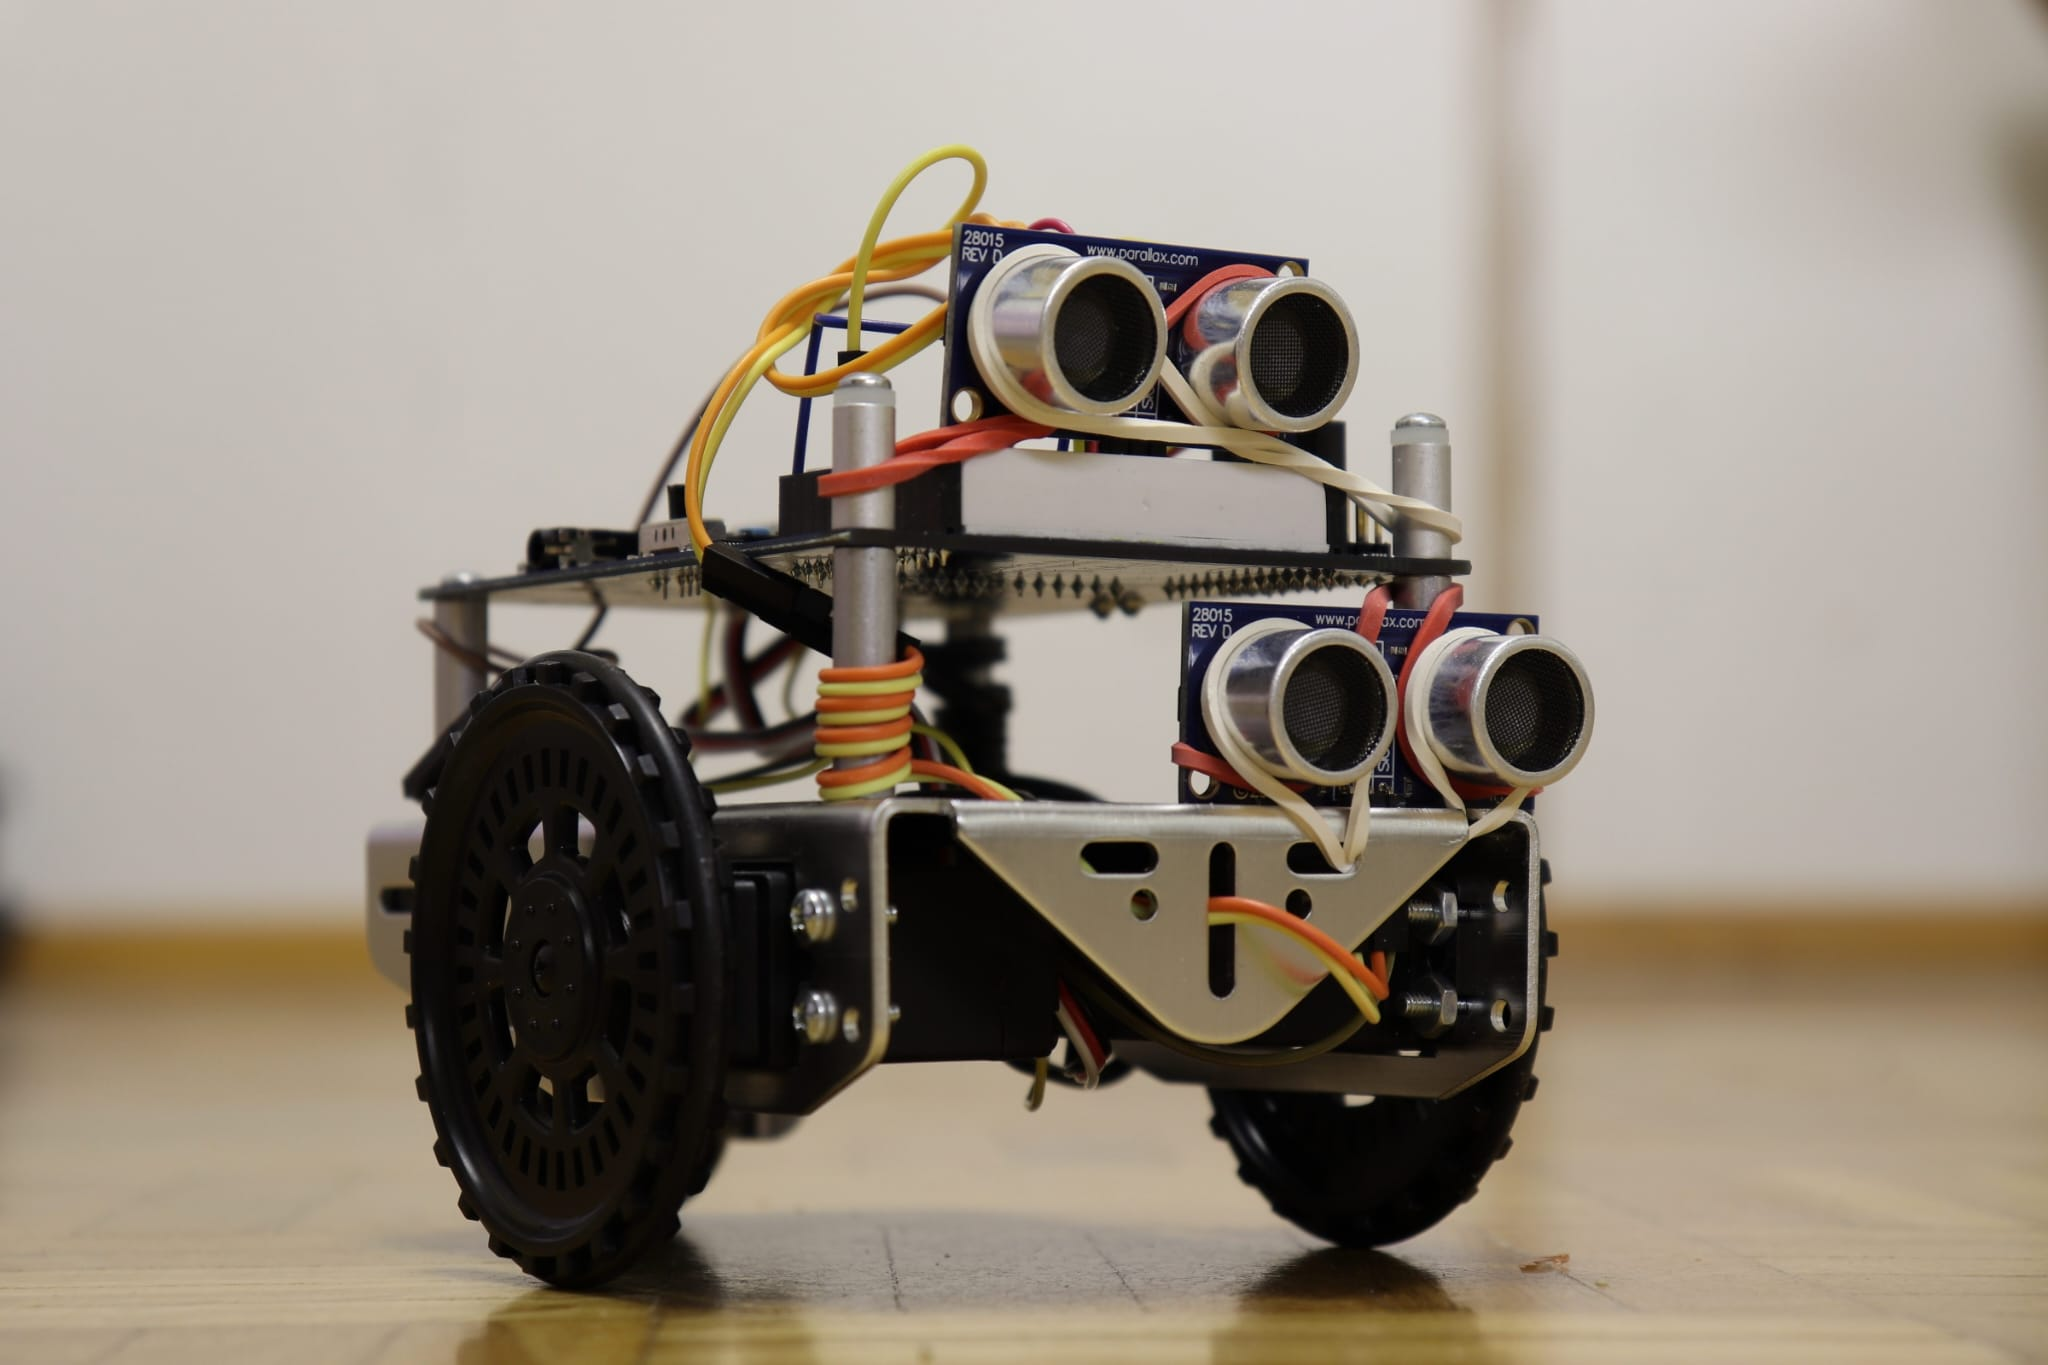
\includegraphics[width=0.9\textwidth]{resources/Seeker_robot/4.jpeg} % first figure itself
      \caption{\label{fig:Seeker}Seeker Robot.}
    \end{minipage}\hfill
    \begin{minipage}{0.45\textwidth}
        \centering
        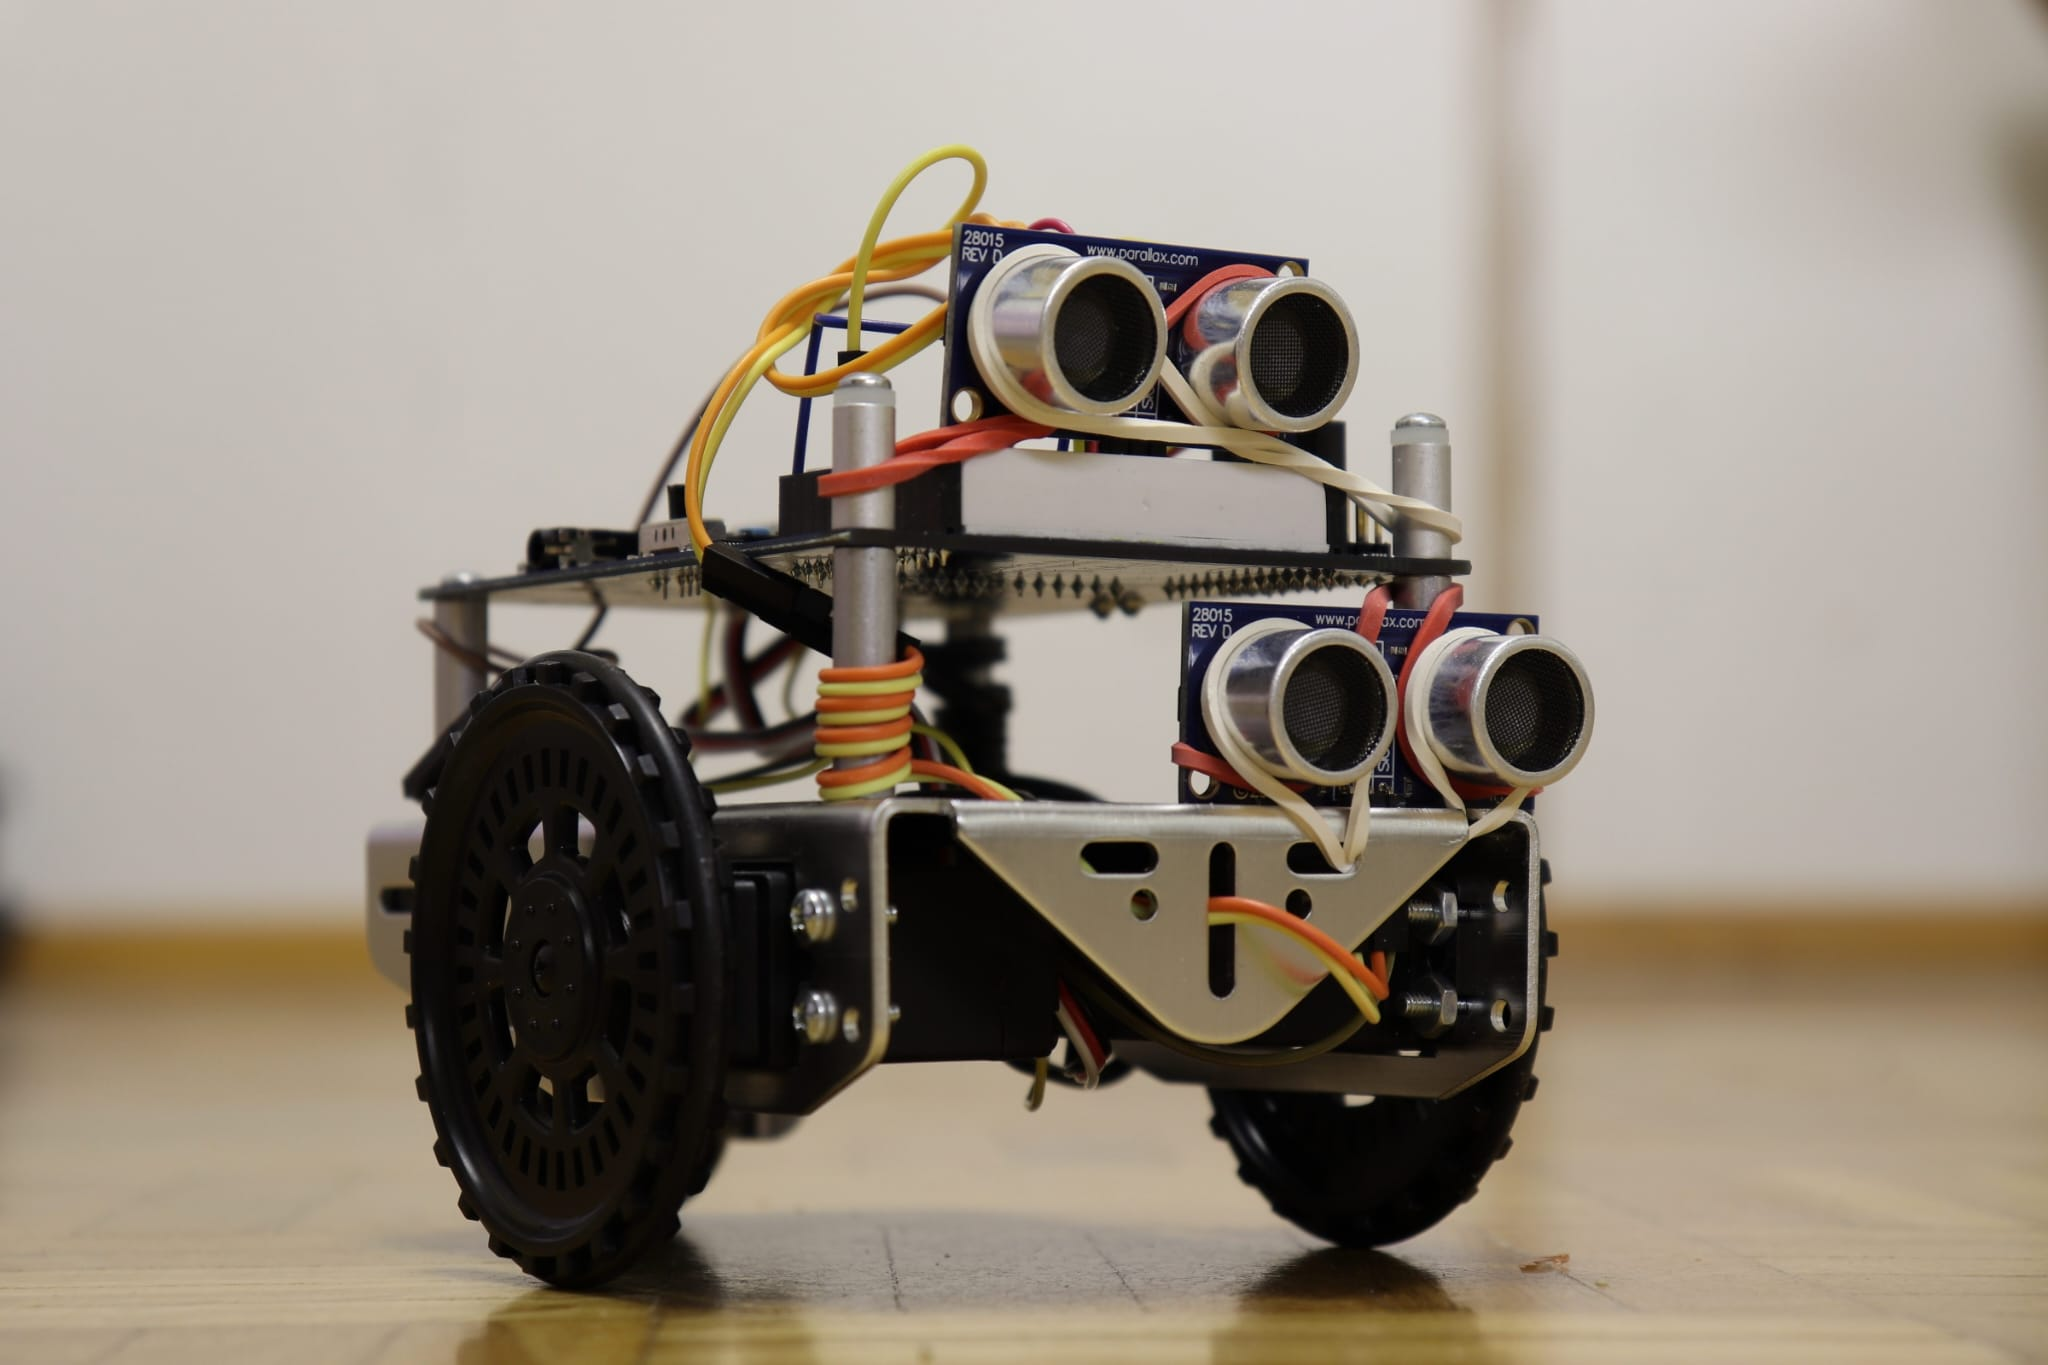
\includegraphics[width=0.9\textwidth]{resources/Seeker_robot/4.jpeg} % second figure itself
      \caption{\label{fig:Runner}Runner Robot. PLACEHOLDER IMG}
    \end{minipage}
\end{figure}


\section{Developing Environment}

      This chapter is meant to explain the working environment of the
      programming
      of Parallax's robots and the work flow that was used throughout this
      project
      

      \subsection{SimpleIDE}

      SimpleIDE is Parallax's official developing platform. As the name
      suggests, it's a rather simple and feature lacking IDE, meant for absolute
      beginners. Basic features like autocompletion, keyword highlight, or even
      error squiggles are not present. This combined with the lack of
      customization makes a more experienced user rather frustrated when trying
      to develop on this platform. 

      \begin{figure}[h]
            \centering
            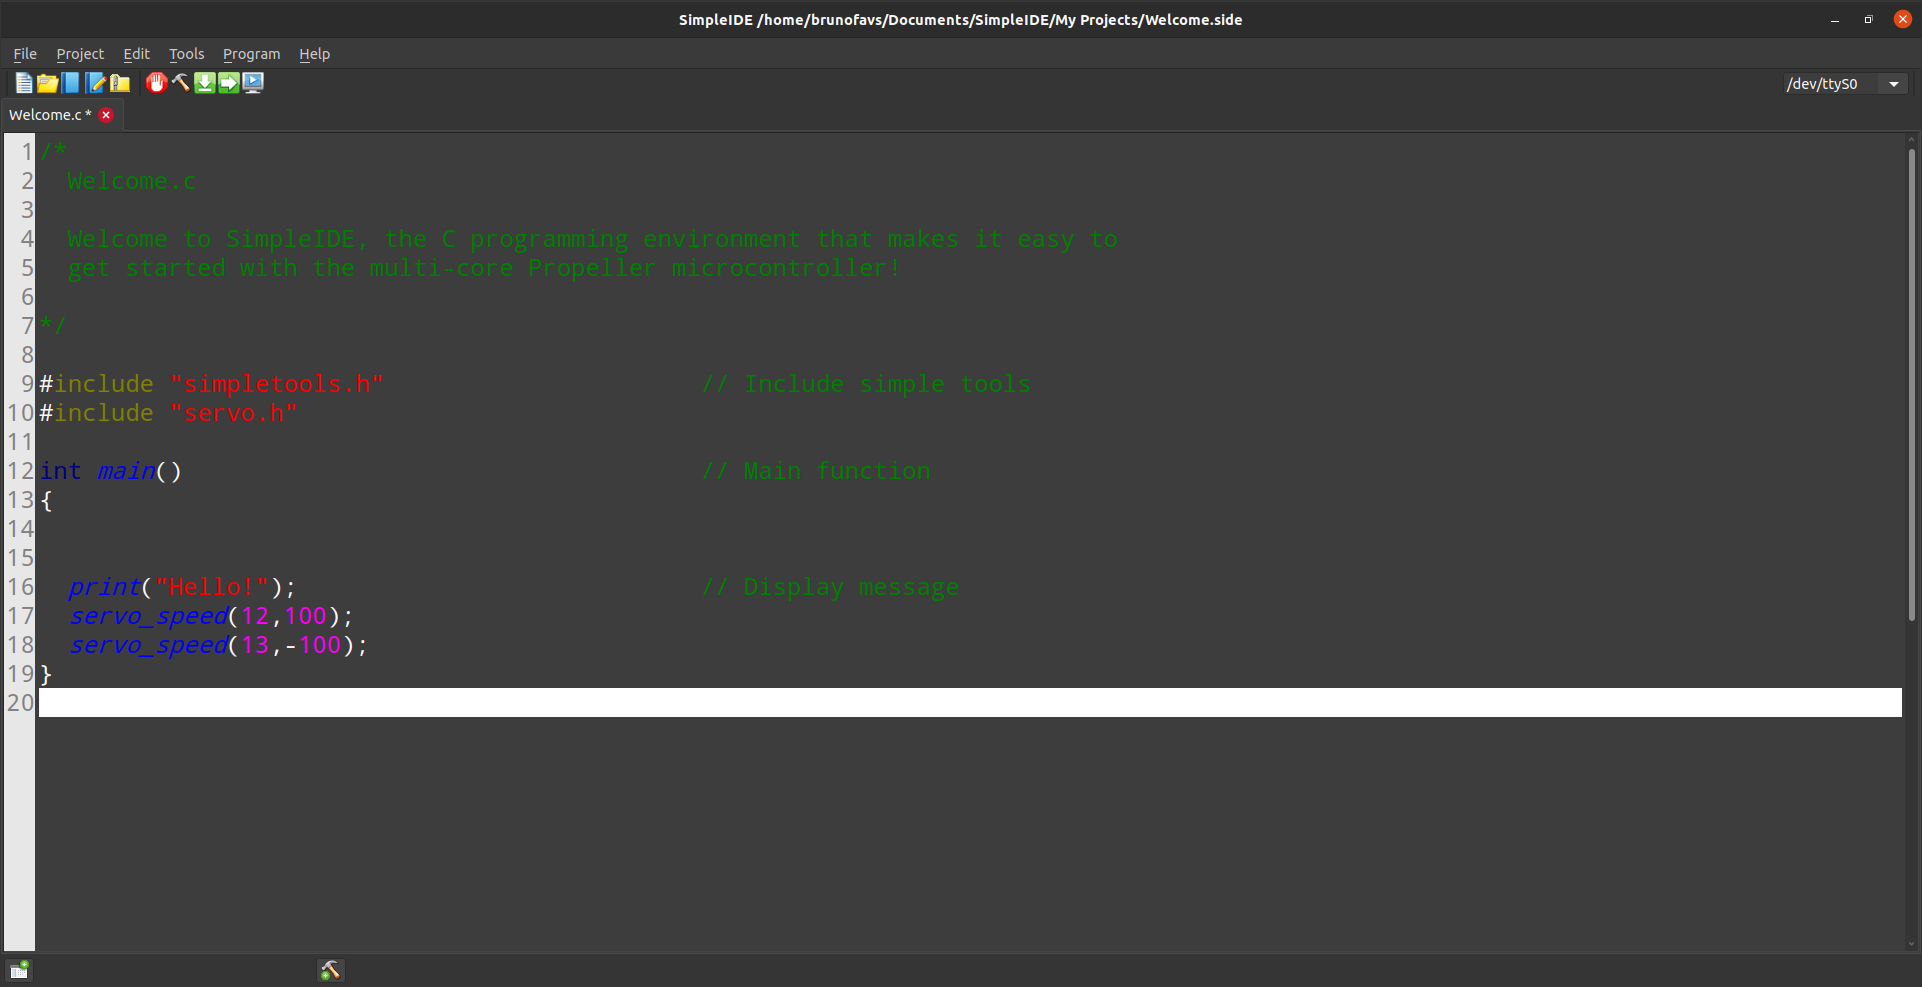
\includegraphics[width=0.8\textwidth]{resources/simple_ide.png}
            \caption{\label{fig:simple_ide}SimpleIDE working environment.}
      \end{figure}



      \subsection{VScode Integration}

      Fortunately, it is possible, with some workarounds, to migrate the grand
      majority of the workflow into a more advanced environment like VScode.
      
      \begin{enumerate}
            \item PlatformIO
                  \begin{itemize}
                        \item PlatformIO's IDE is a VScode
                        extension which transforms VScode into a IDE capable of
                        fully programming a wide range of microcontrollers, from
                        code writting to EEPROM flashing. There's a platform
                        there for working the Parallax's
                        microcontrollers (\href{https://github.com/msquirogac/platform-propeller}{Github}).
                        However, upon exhaustive testing this platform seems to
                        be a half finished attempt which doesn't work.
                  \end{itemize}
            \item VScode
                  \begin{itemize}
                        \item One way is to add SimpleIDE's libraries to the
                        default C path for the default C libraries. This
                        approach is better for long term development, but on
                        this project wasn't used.

                        \item Another way is to import the libraries straight
                        into the project's folder, allowing VScode to treat them
                        as user built libraries.
                        
                        This was the approach used. To replicate the following
                        folders have to be copied to the project folder:
                        \begin{itemize}
                              \item \begin{lstlisting}[language=bash]
$ /home/${USER}/Documents/SimpleIDE/Learn
$ /opt/parallax
                                    \end{lstlisting}
                              \end{itemize}
                              It's important to note that this applies only for Ubuntu
                                    based systems and that both these folders should be
                                    added to the repository's \textit{.gitignore} as they
                                    are quite big and not important to the project itself.
                  \end{itemize}
      \end{enumerate}



\section{Seeker Robot}


\subsection{Algorithm Explanation}

The core of the seeker's algorithm is based on 2 functions:
\begin{enumerate}
      \item Assessing targets in range of ultrasonic sensors;
      
      This involves stopping, getting 2 measurements from each sensor spaced by
      a predefined $\Delta t\space[s]$, calculating the $\Delta d\space[cm]$ from the right and
      left sensor and figure out which direction the target is coming from and
      outputting accordingly.
      \item Giving moving order to the servos to chase the target. This function
      purpose is to, given the direction the target crossed from, tune how much
      the robot should rotate and go forward. This ideally would be dynamically
      controlled, but since the robot cannot know how fast the target crossed,
      it has to be manually tuned for a given target velocity.
\end{enumerate}

\subsection{Function targetAssessing()}

The first thing this function does is assure the robot is still before reading
the differential distance measures. The code could account for the velocity of
the seeker and correct the measure, but that would be mathematically a lot more
challenging.

Then, after reading the distance measurements, the robot could be left with 5
possible case-scenarios given the 2 differential measures :

\begin{enumerate}
     \item $\Delta D_L<0 \wedge \Delta D_R \approx 0$ \\ This would mean the
     target came from out of range and is started being detected the by left
     sensor, since the measure distance reduced. The robot should thus
     turn \textbf{RIGHT};
     
     \item $\Delta D_L\approx 0\wedge \Delta D_R < 0$ \\ This would mean the same
     as case 1, but instead the target is approaching from the right, so the
     robot should turn \textbf{LEFT};

     \item $\Delta D_L>0\wedge \Delta D_R \approx 0$ \\ This would mean the
     target was already in sight of the left sensor and left suddenly to the
     left, allowing the sensor to see into the further away background. This
     would mean the robot should turn \textbf{LEFT};
     
     \item $\Delta D_L\approx 0 \wedge \Delta D_R > 0$ \\ This would mean the
     target was already in sight of the right sensor and left suddenly to the
     right, allowing the sensor to see into the further away background. This
     would mean the robot should turn \textbf{RIGHT};

     \item $|\Delta D_L|>0\wedge |\Delta D_R| > 0$ \\ This would mean that the
     target is currently in front of the robot and is either getting further
     away or getting closer. Either way, for the seeker robot the order should
     be to go \textbf{forward}.
\end{enumerate}

In practice, a \textit{threshold} was used instead of 0, to account for sensor
measurement error.

\begin{figure}[ht]
      \begin{lstlisting}[style = C_style]
            int targetAssessing(){
                  /*
                  This function should assess based on the differential measures whether to turn right or left or keep moving forward
                  0- Go forward
                  1 - Go left
                  2 - Go right
                  */  
            \end{lstlisting}
            \caption{\label{fig:targetAssessing} targetAssessing's
            Function Prototype}
\end{figure}

\subsection{Measuring distances}

In order to assure the robot could always read the latest reading from the
sensor when needing to evaluate distances, and to take advantage of the
parallax's multicore chip, the sensor data is being stored on a global variable
that is constantly being updates parallel to the code. The code for acquiring
data is running on a separate core. 

\begin{lstlisting}[style = C_style]

cog_run(computeDistances,256);

\end{lstlisting}

The following function is used to measure the differential distance measures:
\begin{lstlisting}[style = C_style]

void computeDistances(){
  while(1){
    int first_left = ping_cm(LEFT_SENSOR_PIN); // Measure left sensor
    int first_right = ping_cm(RIGHT_SENSOR_PIN); // Measure right sensor

    pause(10);   // Pause 100ms                     
    
    delta_dist_left = ping_cm(LEFT_SENSOR_PIN) - first_left;
    delta_dist_right = ping_cm(RIGHT_SENSOR_PIN) - first_right;
}
 
\end{lstlisting}


\subsection{Electric Connections}

\section{Runner Robot}

The runner robot, due to lack of sensors, will be running a more primitive
algorithm, sort of permanent blind runner. An initial approach would be
just making the runner go in circles.





\bibliographystyle{alpha}
\bibliography{sample}

\end{document}